Mesmo com o procedimento de eliminação de conjuntos muito similares, a dependência remanescente entre conjuntos teve uma influência quantificável nos resultados.

A dificuldade imposta pelos conjuntos de dados pode ser estimada pela diferença entre os coeficientes de correlação de Spearman de PCT (\textit{Predictive Clustering Trees}) e Def (ranqueamento médio)
para cada metaexemplo.
Assim, é possível comparar o nível de dificuldade oferecido pelos metaexemplos correspondentes a domínios similares  e aquele oferecido pelos demais metaexemplos.
Por simplicidade, foi escolhida apenas uma das melhores estratégias, HTUeuc, neste ensaio.

Na Figura \ref{dsscorr}, a coluna \textit{Valor} indica a diferença de correlações por metaexemplo cujo conjunto de dados correspondente tem seu nome dado na primeira coluna.
\begin{figure}
\centering
% % % números dos cjts de dados errados
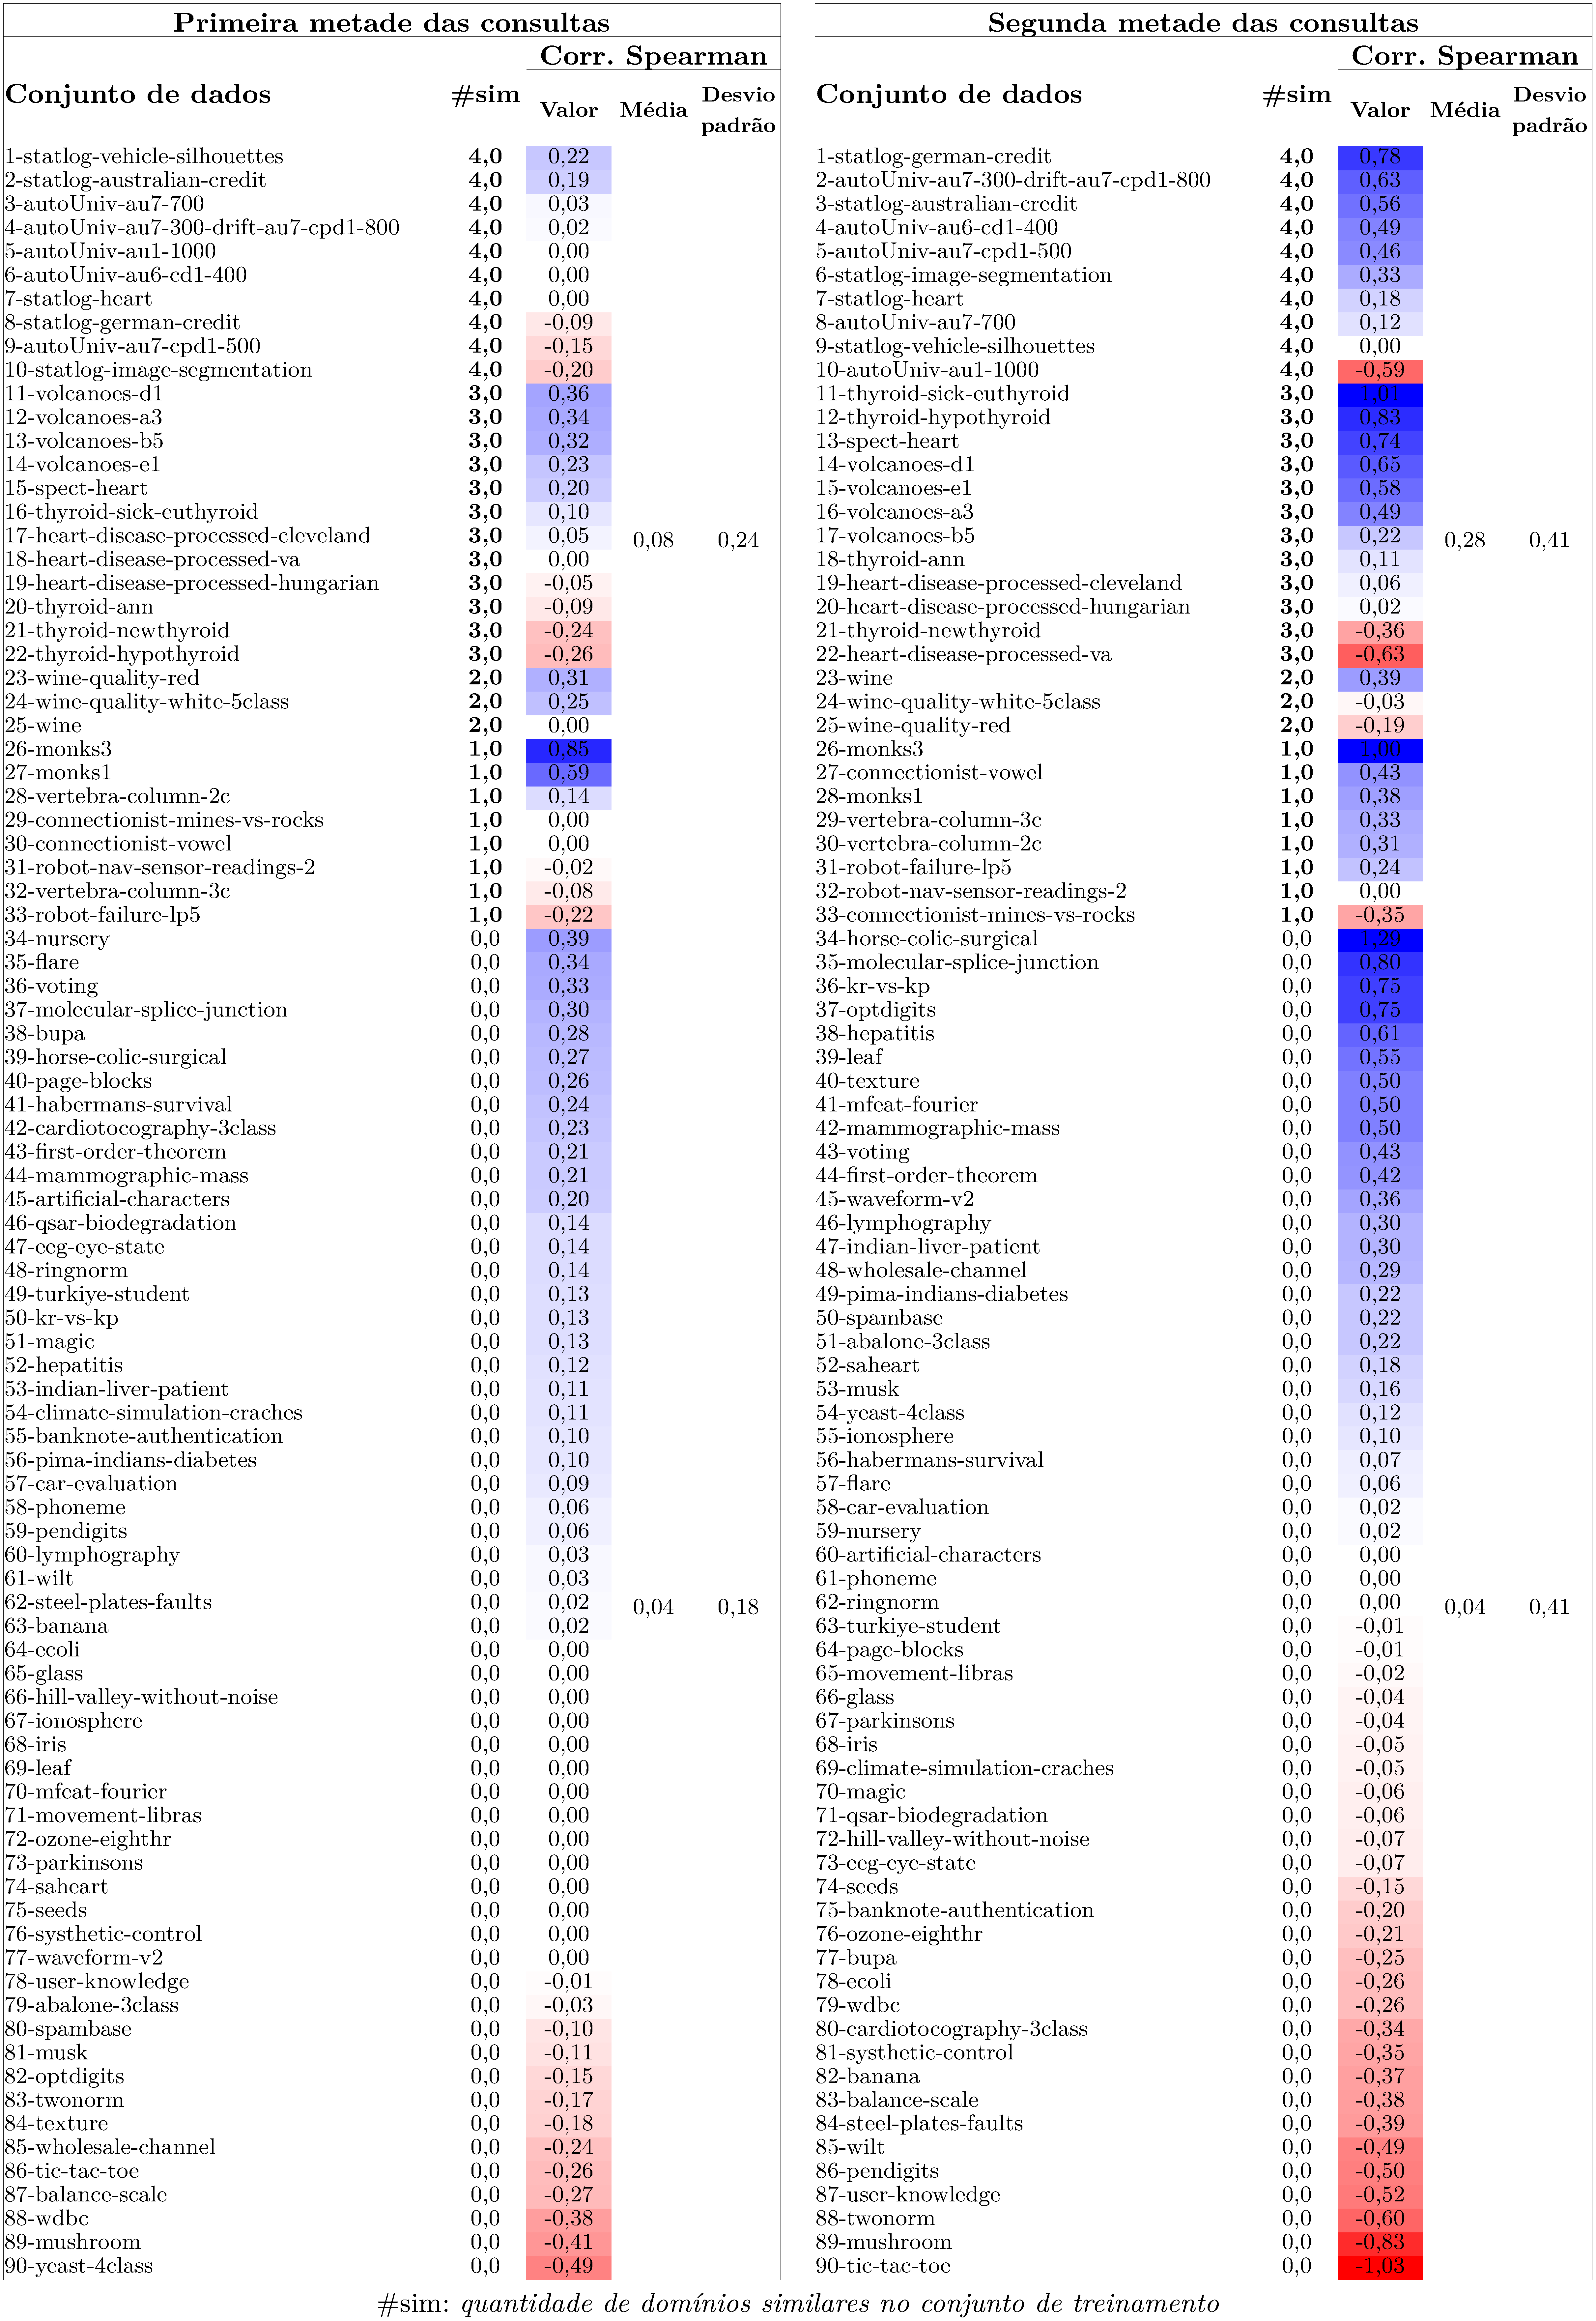
\includegraphics[scale=0.195]{images/dsscorr.pdf}
\caption[Coeficiente de correlação de Spearman por conjunto de dados.]{Coeficiente de correlação de Spearman por conjunto de dados.}
\label{dsscorr}
\end{figure}
A segunda coluna (\textit{\#sim}) contém a quantidade de metaexemplos utilizados para treinamento cujos domínios são similares ao domínio do conjunto de dados indicado na primeira coluna.
A coluna \textit{Média} contém apenas dois valores: a média das diferenças de correlação para os metaexemplos com mais de zero similares no conjunto de treinamento e a média das diferenças de correlações para os demais metaexemplos.

Nas duas metades das consultas, o maior valor médio das diferenças de correlações ocorreu para os metaexemplos com maior quantidade de similares: na primeira metade, 0,08 contra 0,04; e, na segunda metade, 0,28 contra 0,04.
Isso sugere que a coleção de conjuntos adotada possa ter elevado as medidas de desempenho por conta da existência de dependência entre as amostras (conjuntos de dados).
Apesar disso, a média das diferenças entre PCT e Def ainda é positiva nas duas metades, indicando um desempenho acima da referência, mesmo em metaexemplos correspondentes a domínios independentes, isto é, sem similar no conjunto de treinamento.
Embora a presença de domínios similares facilite a tarefa de recomendação, ela não reduz a necessidade do sistema de recomendação, apenas sugere que ele seja, naturalmente, mais efetivo em coleções que contenham conjuntos de domínios similares ao do conjunto que se pretenda rotular.
